%!TEX TS-program = xelatex
%!TEX encoding = UTF-8 Unicode

\documentclass[11pt,tikz,border=1]{standalone}
\usepackage{pgfplots}
\usetikzlibrary{positioning}

\begin{document}
  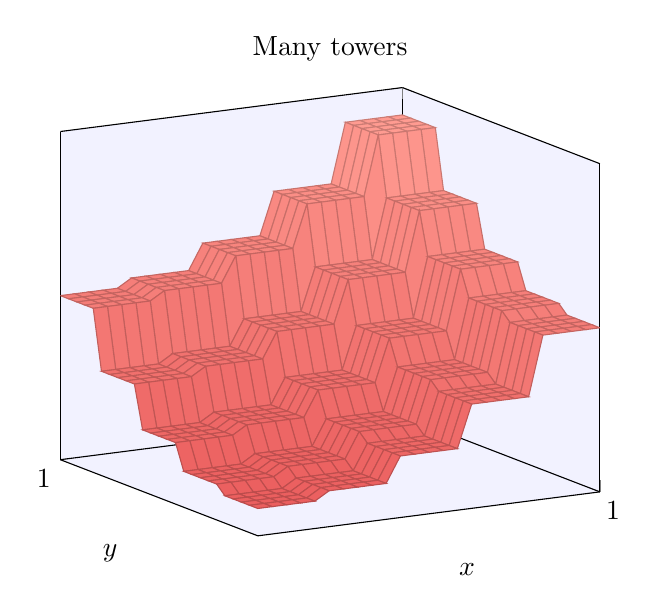
\begin{tikzpicture}[
    neuron/.style={circle,draw,inner sep=0pt,minimum size=10mm}
    ]
    
      \begin{axis}[
        view={-30}{15},        
        axis background/.style={fill=blue!5},
        xlabel=$x$,
        ylabel=$y$,
        xtick distance=1,
        ytick distance=1,
        ztick distance=1,
        xtick={1},
        ytick={1},
        ztick={2},  % big number to disable
        title={Many towers},
        colormap={simple}{rgb255=(235,95,95) rgb255=(255,155,145)},
        declare function={
        	g(\z)=floor(\z * 4.999);
        	f(\x,\y)=(g(\x)*g(\x) + g(\y) * g(\y))/50;
       }]
        \addplot3[surf,domain=0:1] {
        	f(x,y)
        };
      \end{axis}
    
  \end{tikzpicture} 
\end{document}
